\section{PLATOSim}
PLATOSim is a Simulator developed by the University Leuven which generates data as the PLATO mission will do, by simulating the whole acquisition process. The process aims to synthesize the satellite images as realisticly as possible by including all known noise sources and generating a numerically modelled imagette for each considered star. 
\newline
PLATOSim is planned to be a tool for the scientific comunity which is easily adaptable for other high-precision photometric space missions as well, therefore it is build very versatile and easy tweakable in its parameters.
\newline
In this section the architecture and the mode of operation of the tool and all considered influence parameters are described.
\subsection{Input and Output}

\subsection{Simulation Process}  
The working process of PLATOSim is shown in figure \ref{fig:mesh1}. In this section The single steps are shown and analysed for their relevance for the fine guidance system.
\newline

\begin{figure}[h]
\centering
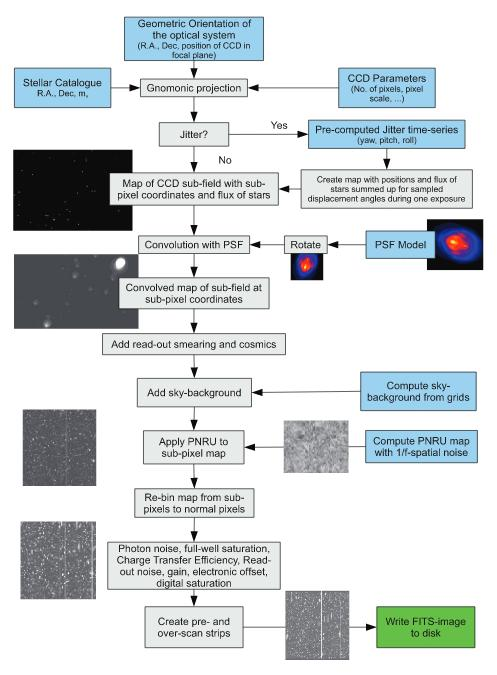
\includegraphics[width=\textwidth]{PLATOSim_Ablauf.jpg}
\caption{PLATOSim process}
\label{fig:mesh1}
\end{figure}

PLATOSim aims to generate only one imagette for one star with one exposure of the camera at the time. The whole CCD is generally not calculated because of the high memory consumption, which would be needed for such a task. Instead only the small section, where the light of the specific star falls on the CCD is simulated.
\newline
To correctly simulate motions and noise effects even the relatively small size (18 mycrometer) of the pixels is too large. Therefore it is necessary to subdivide each physical pixel in a number of subpixels to display intra-pixel sensitivities. The aforementioned imagette is enlarged in its dimensions depending on the number of subpixels the user wishes. All effects like the PSF or noise sources are applied on this subpixelmap, before it's rebinned again to the small imagette in the end. The more subpixels are used, the more accurate the result will be in theory.  However a larger subpixel map comes always at the price of longer processing times and more needed memory. 

\subsubsection{Geometry}
The first step is to determine where a star falls on which CCD of a camera. Therefore a few input data are required. The most important ones are the information about the currently relevant star and the orientation of the pointing axis of the satellite. 